\documentclass{beamer}
\usepackage[utf8]{inputenc}

\usetheme{Madrid}
\usecolortheme{default}
\usepackage{amsmath,amssymb,amsfonts,amsthm}
\usepackage{txfonts}
\usepackage{tkz-euclide}
\usepackage{listings}
\usepackage{adjustbox}
\usepackage{array}
\usepackage{tabularx}
\usepackage{gvv}
\usepackage{lmodern}
\usepackage{circuitikz}
\usepackage{tikz}
\usepackage{graphicx}

\setbeamertemplate{page number in head/foot}[totalframenumber]

\title 
{1.8.20}
\date{September 7,2025}

\author 
{ADHARVAN KSHATHRIYA BOMMAGANI - EE25BTECH11003}

\begin{document}

\frame{\titlepage}

% Question Slide
\begin{frame}{Question}
Find a relation between $x$ and $y$ such that the point $(x,y)$ is equidistant from the point $(3,6)$ and $(-3,4)$.
\end{frame}

% Step 1: Define Points
\begin{frame}{Theoritical Solution}
\begin{align}
\vec{A} = \myvec{3 \\ 6}, \quad
\vec{B} = \myvec{-3 \\ 4}
\end{align}

Midpoint of $AB$:
\begin{align}
\vec{M} = \frac{\vec{A}+\vec{B}}{2}
= \myvec{0 \\ 5}
\end{align}

Let a general point on the perpendicular bisector be
\begin{align}
\vec{P} = \myvec{x \\ y}
\end{align}
\end{frame}

% Step 2: Perpendicular condition
\begin{frame}{Theoritical Solution}
\begin{align}
\vec{P}-\vec{M} &= \myvec{x \\ y-5}
\end{align}

Perpendicular condition:
\begin{align}
(\vec{P}-\vec{M})^T (\vec{B}-\vec{A}) = 0
\end{align}

\begin{align}
\myvec{x & y-5}\myvec{-6 \\ -2} = 0
\end{align}
\end{frame}

% Step 3: Simplification
\begin{frame}{Theoritical Solution}
\begin{align}
-6x - 2y + 10 = 0
\end{align}
\begin{align}
3x + y = 5
\end{align}

\[
\therefore \quad \text{The required relation is } 3x+y=5.
\]
\end{frame}

\begin{frame}[fragile]
    \frametitle{Python Code}
    \begin{lstlisting}

import matplotlib.pyplot as plt
import numpy as np

# Points
A = (3, 6)
B = (-3, 4)
M = ((A[0] + B[0]) / 2, (A[1] + B[1]) / 2)

# Plot line segment AB
plt.plot([A[0], B[0]], [A[1], B[1]], 'b-', label='Line segment AB')

# Plot points A, B, and M
plt.scatter(*A, color='red', label='A(3,6)')
plt.scatter(*B, color='green', label='B(-3,4)')
plt.scatter(*M, color='purple', marker='x', s=100, label='Midpoint M(0,5)')

\end{lstlisting}
\end{frame}

\begin{frame}[fragile]
    \frametitle{Python Code}
    \begin{lstlisting}

# Annotate points
plt.text(A[0]+0.2, A[1], 'A(3,6)', fontsize=10)
plt.text(B[0]-1, B[1]-0.3, 'B(-3,4)', fontsize=10)
plt.text(M[0]+0.2, M[1], 'M(0,5)', fontsize=10, color='purple')

# Perpendicular bisector: y = 5 - 3x
x_vals = np.linspace(-5, 5, 400)
y_vals = 5 - 3*x_vals
plt.plot(x_vals, y_vals, 'r--', label='Perpendicular bisector (y+3x=5)')

# Axes, grid, legend
plt.axhline(0, color='black', linewidth=0.8)
plt.axvline(0, color='black', linewidth=0.8)
plt.grid(True, linestyle='--', alpha=0.6)
plt.legend()

\end{lstlisting}
\end{frame}

\begin{frame}[fragile]
    \frametitle{Python Code}
    \begin{lstlisting}
plt.title("Line Segment AB with Midpoint M and Perpendicular Bisector")
plt.xlabel("x-axis")
plt.ylabel("y-axis")
plt.axis('equal')

plt.show()

\end{lstlisting}
\end{frame}
\begin{frame}[fragile]
    \frametitle{C Code}
    \begin{lstlisting}
#include <stdio.h>


float perpendicularSlope(float x1, float y1, float x2, float y2) {
    float slope;

    
    if (x2 - x1 == 0) {
        
        return 0.0;  
    }

   
        
       
    \end{lstlisting}
\end{frame}

\begin{frame}[fragile]
    \frametitle{C Code}
    \begin{lstlisting}
    if (y2 - y1 == 0) {
        return 9999999.0;
    }
    
    slope = (y2 - y1) / (x2 - x1);
   return -1.0 / slope;
}
\end{lstlisting}
\end{frame}


 \begin{frame}[fragile]
 \frametitle{Python Code}
 \begin{lstlisting}
import ctypes
import sys
import matplotlib.pyplot as plt

# Load the compiled shared library
lib = ctypes.CDLL("./libslope.so")

# Define the argument and return types for the C function
lib.perpendicularSlope.argtypes = [ctypes.c_float, ctypes.c_float, ctypes.c_float, ctypes.c_float]
lib.perpendicularSlope.restype = ctypes.c_float
\end{lstlisting}
\end{frame}

 \begin{frame}[fragile]
 \frametitle{Python Code}
 \begin{lstlisting}
# Input points
x1, y1 = 3.0, 6.0
x2, y2 = -3.0, 4.0

# Call the C function
perp_slope = lib.perpendicularSlope(x1, y1, x2, y2)

\end{lstlisting}
\end{frame}

 \begin{frame}[fragile]
 \frametitle{Python Code}
 \begin{lstlisting}
# Print the perpendicular slope
if perp_slope == 9999999.0:
    print("The perpendicular line is vertical (slope undefined).")
else:
    print(f"The slope of the perpendicular line is: {perp_slope:.2f}")

# Plot the original line connecting (x1, y1) and (x2, y2)
plt.figure(figsize=(6, 6))
plt.plot([x1, x2], [y1, y2], 'b-o', label='Line Joining Points')

# Highlight the two points
plt.scatter([x1, x2], [y1, y2], color='red')
plt.text(x1, y1, f"({x1}, {y1})", fontsize=10, ha='right')
plt.text(x2, y2, f"({x2}, {y2})", fontsize=10, ha='right')
\end{lstlisting}
\end{frame}

 \begin{frame}[fragile]
 \frametitle{Python Code}
 \begin{lstlisting}
# Midpoint
mid_x = (x1 + x2) / 2.0
mid_y = (y1 + y2) / 2.0
plt.scatter(mid_x, mid_y, color='green', label='Midpoint')
plt.text(mid_x, mid_y, f"({mid_x:.1f}, {mid_y:.1f})", fontsize=10, ha='left')

# Add labels and grid
plt.xlabel("X-axis")
plt.ylabel("Y-axis")
plt.title("Line Joining Two Points")
plt.grid(True)
plt.legend()
plt.axis('equal')

# Show the plot
plt.show()

\end{lstlisting}
\end{frame}
\begin{frame}
    \vspace{5em}
\textbf{Graph of line segment AB with midpoint M and perpendicular bisector}
\begin{figure}[H]
    \centering
    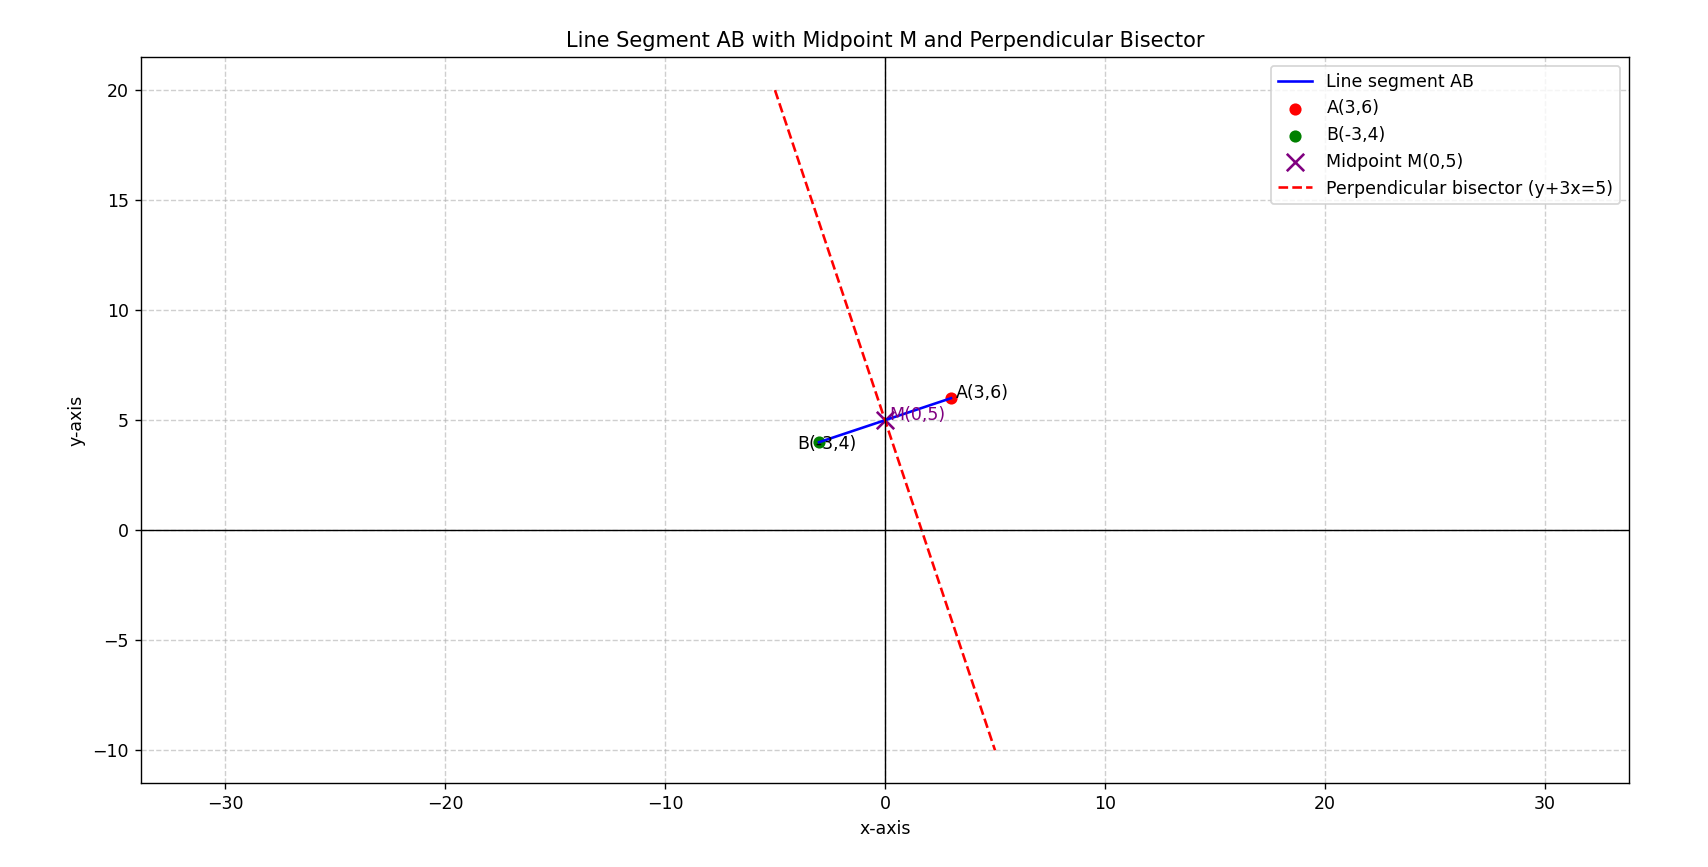
\includegraphics[width=0.75\columnwidth]{figs/fig1.png}
    \caption{Figure for 1.8.20}
    \label{fig1}
\end{figure}
\end{frame}

\end{document}
